% !TEX root = ./main.tex
\begin{figure}[h]
    \centering
    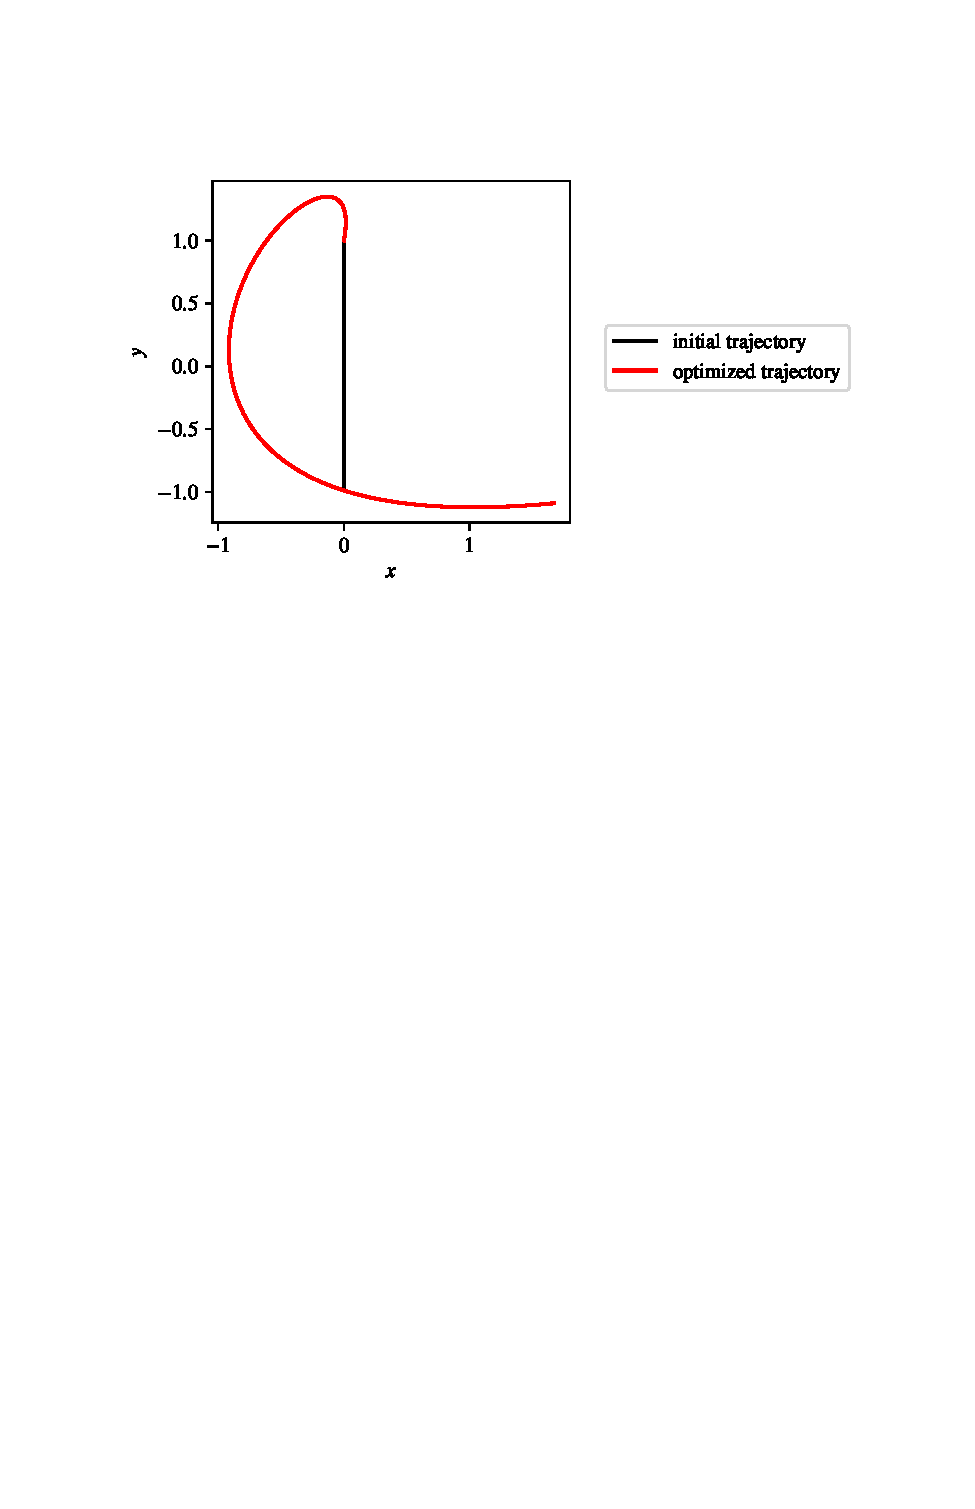
\includegraphics[width=\textwidth]{hw5_1.pdf}
    \vspace{-5mm}
    \caption{Plot of the maximally ergodic trajectory found using my implementation. 
    Compared to the initial trajectory, the optimized one definitively shows better coverage with respect to the given Gaussian distribution, 
    but it is evidently still not completely covering the entire domain. Especially, the found trajectory does not cover the mode of the Gaussian.}
    \label{fig:ergodic}
\end{figure}
\begin{figure}[h]
    \centering
    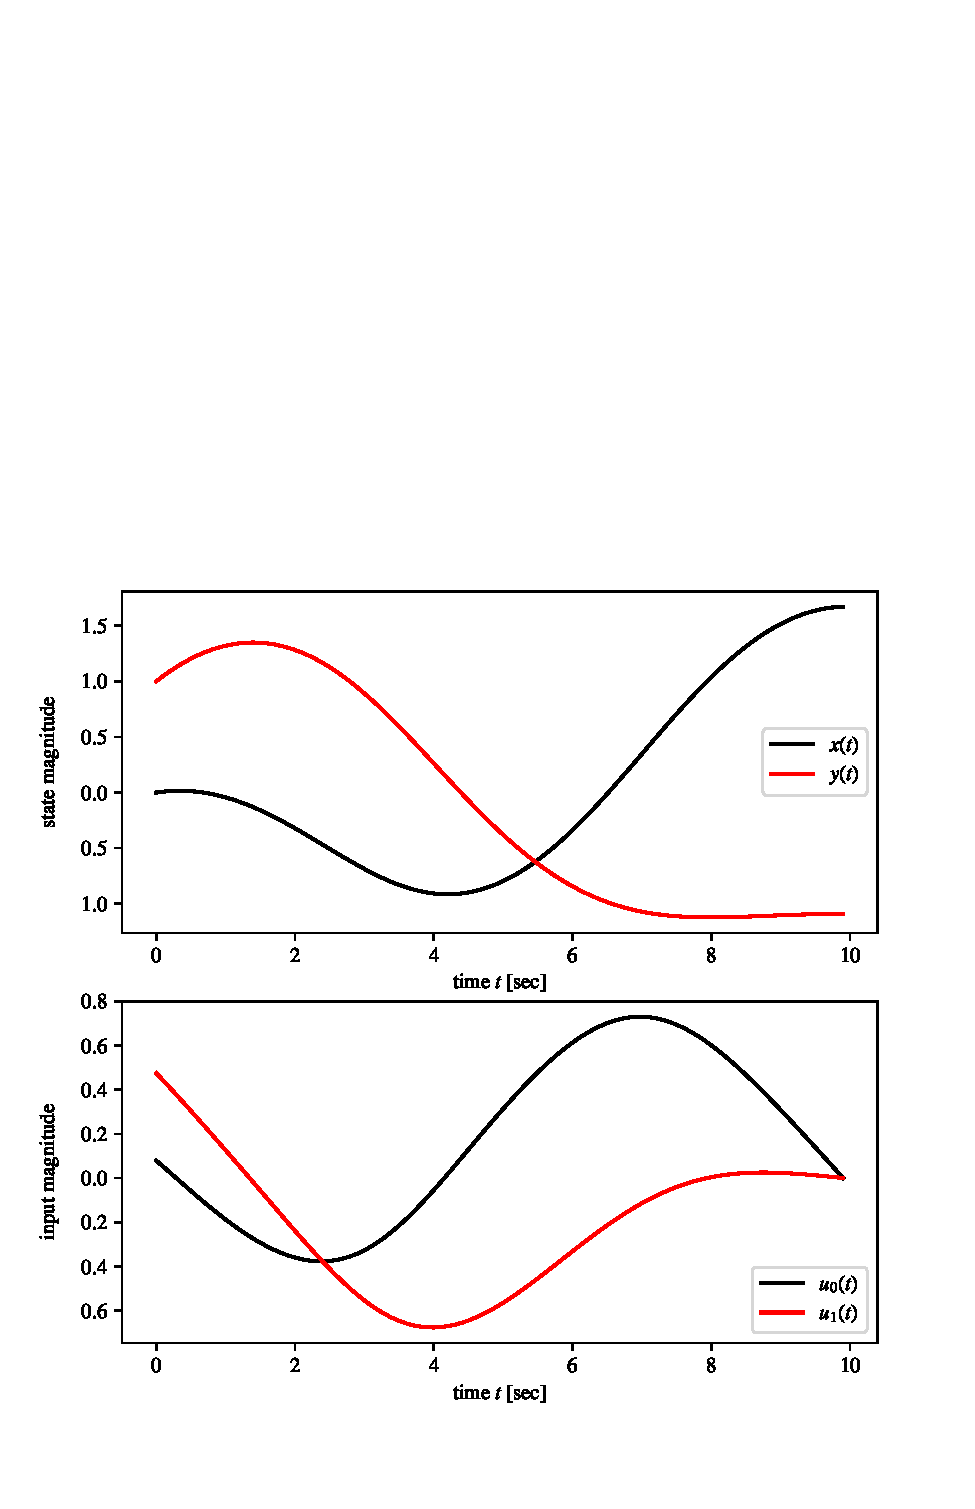
\includegraphics[]{hw5.pdf}
    \vspace{-5mm}
    \caption{Plot of the optimized state and input trajectory over time.}
    \label{fig:ergodic_time}
\end{figure}
\begin{figure}[h]
    \centering
    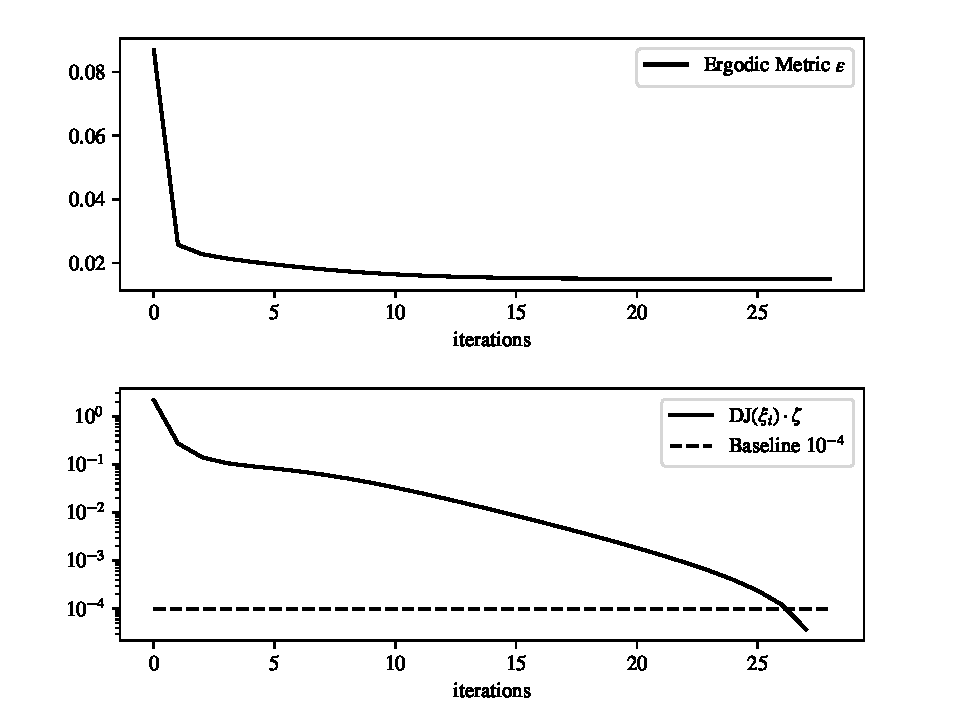
\includegraphics[]{hw5_convergence.pdf}
    \vspace{-5mm}
    \caption{Convergence of Cost Derivative DJ$(\xi_i)\cdot\zeta$}
    \label{fig:convergence}
\end{figure}
% Is there a most ergodic choice of b? 
% What is the most ergodic choice if you can choose both b and the time horizon T?
The optimized trajectory as seen in the figure above was found using an implementation of the \textit{Ergodic Exploration} algorithm as seen in the lecture notes.
As for hyperparameters, a choice of $k=5$ coefficients in each dimension and integrating for the spatial distribution coefficients over the domain $[-5,5]\times[-5,5]$ was made. 
The cost function matrices used were $q=5$, $Q=\textrm{diag}(0.1,0.1)$, $R=\textrm{diag}(0.1,0.1)$. The step size was fixed at $\gamma = 0.01.$

Comparing to benchmarks such as \url{https://arxiv.org/pdf/1808.06652.pdf}, the implemented algorithm is still relatively far from finding a truly maximally ergodic trajectory. 
Regrettably, I did not manage to find any more bugs in my code. Please refer to my implementation here: \url{https://github.com/Bakeey/active-learning/blob/main/hw5/main.py}